% Options for packages loaded elsewhere
\PassOptionsToPackage{unicode}{hyperref}
\PassOptionsToPackage{hyphens}{url}
%
\documentclass[
  ignorenonframetext,
]{beamer}
\usepackage{pgfpages}
\setbeamertemplate{caption}[numbered]
\setbeamertemplate{caption label separator}{: }
\setbeamercolor{caption name}{fg=normal text.fg}
\beamertemplatenavigationsymbolsempty
% Prevent slide breaks in the middle of a paragraph
\widowpenalties 1 10000
\raggedbottom
\setbeamertemplate{part page}{
  \centering
  \begin{beamercolorbox}[sep=16pt,center]{part title}
    \usebeamerfont{part title}\insertpart\par
  \end{beamercolorbox}
}
\setbeamertemplate{section page}{
  \centering
  \begin{beamercolorbox}[sep=12pt,center]{part title}
    \usebeamerfont{section title}\insertsection\par
  \end{beamercolorbox}
}
\setbeamertemplate{subsection page}{
  \centering
  \begin{beamercolorbox}[sep=8pt,center]{part title}
    \usebeamerfont{subsection title}\insertsubsection\par
  \end{beamercolorbox}
}
\AtBeginPart{
  \frame{\partpage}
}
\AtBeginSection{
  \ifbibliography
  \else
    \frame{\sectionpage}
  \fi
}
\AtBeginSubsection{
  \frame{\subsectionpage}
}
\usepackage{lmodern}
\usepackage{amssymb,amsmath}
\usepackage{ifxetex,ifluatex}
\ifnum 0\ifxetex 1\fi\ifluatex 1\fi=0 % if pdftex
  \usepackage[T1]{fontenc}
  \usepackage[utf8]{inputenc}
  \usepackage{textcomp} % provide euro and other symbols
\else % if luatex or xetex
  \usepackage{unicode-math}
  \defaultfontfeatures{Scale=MatchLowercase}
  \defaultfontfeatures[\rmfamily]{Ligatures=TeX,Scale=1}
\fi
% Use upquote if available, for straight quotes in verbatim environments
\IfFileExists{upquote.sty}{\usepackage{upquote}}{}
\IfFileExists{microtype.sty}{% use microtype if available
  \usepackage[]{microtype}
  \UseMicrotypeSet[protrusion]{basicmath} % disable protrusion for tt fonts
}{}
\makeatletter
\@ifundefined{KOMAClassName}{% if non-KOMA class
  \IfFileExists{parskip.sty}{%
    \usepackage{parskip}
  }{% else
    \setlength{\parindent}{0pt}
    \setlength{\parskip}{6pt plus 2pt minus 1pt}}
}{% if KOMA class
  \KOMAoptions{parskip=half}}
\makeatother
\usepackage{xcolor}
\IfFileExists{xurl.sty}{\usepackage{xurl}}{} % add URL line breaks if available
\IfFileExists{bookmark.sty}{\usepackage{bookmark}}{\usepackage{hyperref}}
\hypersetup{
  pdftitle={Module 4: Introduction to the Normal Gamma Model},
  pdfauthor={Rebecca C. Steorts and Lei Qian},
  hidelinks,
  pdfcreator={LaTeX via pandoc}}
\urlstyle{same} % disable monospaced font for URLs
\newif\ifbibliography
\usepackage{color}
\usepackage{fancyvrb}
\newcommand{\VerbBar}{|}
\newcommand{\VERB}{\Verb[commandchars=\\\{\}]}
\DefineVerbatimEnvironment{Highlighting}{Verbatim}{commandchars=\\\{\}}
% Add ',fontsize=\small' for more characters per line
\usepackage{framed}
\definecolor{shadecolor}{RGB}{248,248,248}
\newenvironment{Shaded}{\begin{snugshade}}{\end{snugshade}}
\newcommand{\AlertTok}[1]{\textcolor[rgb]{0.94,0.16,0.16}{#1}}
\newcommand{\AnnotationTok}[1]{\textcolor[rgb]{0.56,0.35,0.01}{\textbf{\textit{#1}}}}
\newcommand{\AttributeTok}[1]{\textcolor[rgb]{0.77,0.63,0.00}{#1}}
\newcommand{\BaseNTok}[1]{\textcolor[rgb]{0.00,0.00,0.81}{#1}}
\newcommand{\BuiltInTok}[1]{#1}
\newcommand{\CharTok}[1]{\textcolor[rgb]{0.31,0.60,0.02}{#1}}
\newcommand{\CommentTok}[1]{\textcolor[rgb]{0.56,0.35,0.01}{\textit{#1}}}
\newcommand{\CommentVarTok}[1]{\textcolor[rgb]{0.56,0.35,0.01}{\textbf{\textit{#1}}}}
\newcommand{\ConstantTok}[1]{\textcolor[rgb]{0.00,0.00,0.00}{#1}}
\newcommand{\ControlFlowTok}[1]{\textcolor[rgb]{0.13,0.29,0.53}{\textbf{#1}}}
\newcommand{\DataTypeTok}[1]{\textcolor[rgb]{0.13,0.29,0.53}{#1}}
\newcommand{\DecValTok}[1]{\textcolor[rgb]{0.00,0.00,0.81}{#1}}
\newcommand{\DocumentationTok}[1]{\textcolor[rgb]{0.56,0.35,0.01}{\textbf{\textit{#1}}}}
\newcommand{\ErrorTok}[1]{\textcolor[rgb]{0.64,0.00,0.00}{\textbf{#1}}}
\newcommand{\ExtensionTok}[1]{#1}
\newcommand{\FloatTok}[1]{\textcolor[rgb]{0.00,0.00,0.81}{#1}}
\newcommand{\FunctionTok}[1]{\textcolor[rgb]{0.00,0.00,0.00}{#1}}
\newcommand{\ImportTok}[1]{#1}
\newcommand{\InformationTok}[1]{\textcolor[rgb]{0.56,0.35,0.01}{\textbf{\textit{#1}}}}
\newcommand{\KeywordTok}[1]{\textcolor[rgb]{0.13,0.29,0.53}{\textbf{#1}}}
\newcommand{\NormalTok}[1]{#1}
\newcommand{\OperatorTok}[1]{\textcolor[rgb]{0.81,0.36,0.00}{\textbf{#1}}}
\newcommand{\OtherTok}[1]{\textcolor[rgb]{0.56,0.35,0.01}{#1}}
\newcommand{\PreprocessorTok}[1]{\textcolor[rgb]{0.56,0.35,0.01}{\textit{#1}}}
\newcommand{\RegionMarkerTok}[1]{#1}
\newcommand{\SpecialCharTok}[1]{\textcolor[rgb]{0.00,0.00,0.00}{#1}}
\newcommand{\SpecialStringTok}[1]{\textcolor[rgb]{0.31,0.60,0.02}{#1}}
\newcommand{\StringTok}[1]{\textcolor[rgb]{0.31,0.60,0.02}{#1}}
\newcommand{\VariableTok}[1]{\textcolor[rgb]{0.00,0.00,0.00}{#1}}
\newcommand{\VerbatimStringTok}[1]{\textcolor[rgb]{0.31,0.60,0.02}{#1}}
\newcommand{\WarningTok}[1]{\textcolor[rgb]{0.56,0.35,0.01}{\textbf{\textit{#1}}}}
\usepackage{graphicx,grffile}
\makeatletter
\def\maxwidth{\ifdim\Gin@nat@width>\linewidth\linewidth\else\Gin@nat@width\fi}
\def\maxheight{\ifdim\Gin@nat@height>\textheight\textheight\else\Gin@nat@height\fi}
\makeatother
% Scale images if necessary, so that they will not overflow the page
% margins by default, and it is still possible to overwrite the defaults
% using explicit options in \includegraphics[width, height, ...]{}
\setkeys{Gin}{width=\maxwidth,height=\maxheight,keepaspectratio}
% Set default figure placement to htbp
\makeatletter
\def\fps@figure{htbp}
\makeatother
\setlength{\emergencystretch}{3em} % prevent overfull lines
\providecommand{\tightlist}{%
  \setlength{\itemsep}{0pt}\setlength{\parskip}{0pt}}
\setcounter{secnumdepth}{-\maxdimen} % remove section numbering
% Custom definitions
% To use this customization file, insert the line "% Custom definitions
% To use this customization file, insert the line "% Custom definitions
% To use this customization file, insert the line "% Custom definitions
% To use this customization file, insert the line "\input{custom}" in the header of the tex file.

% Formatting

\tolerance=1000
\usepackage[margin=1in]{geometry}


% Packages

% \usepackage{amssymb,latexsym}
\usepackage{amssymb,amsfonts,amsmath,latexsym,amsthm}
\usepackage[usenames,dvipsnames]{color}
\usepackage[]{graphicx}
\usepackage[space]{grffile}
\usepackage{mathrsfs}   % fancy math font
% \usepackage[font=small,skip=0pt]{caption}
\usepackage[skip=0pt]{caption}
\usepackage{subcaption}
\usepackage{verbatim}
\usepackage{url}
\usepackage{bm}
\usepackage{dsfont}
\usepackage{extarrows}
\usepackage{multirow}
% \usepackage{wrapfig}
% \usepackage{epstopdf}
\usepackage{rotating}
\usepackage{tikz}
\usetikzlibrary{fit}					% fitting shapes to coordinates
%\usetikzlibrary{backgrounds}	% drawing the background after the foreground


% \usepackage[dvipdfm,colorlinks,citecolor=blue,linkcolor=blue,urlcolor=blue]{hyperref}
\usepackage[colorlinks,citecolor=blue,linkcolor=blue,urlcolor=blue]{hyperref}
%\usepackage{hyperref}
\usepackage[authoryear,round]{natbib}


%  Theorems, etc.

\theoremstyle{plain}
\newtheorem{theorem}{Theorem}[section]
\newtheorem{corollary}[theorem]{Corollary}
\newtheorem{lemma}[theorem]{Lemma}
\newtheorem{proposition}[theorem]{Proposition}
\newtheorem{condition}[theorem]{Condition}
% \newtheorem{conditions}[theorem]{Conditions}

\theoremstyle{definition}
\newtheorem{definition}[theorem]{Definition}
% \newtheorem*{unnumbered-definition}{Definition}
\newtheorem{example}[theorem]{Example}
\theoremstyle{remark}
\newtheorem*{remark}{Remark}
\numberwithin{equation}{section}




% Document-specific shortcuts
\newcommand{\btheta}{{\bm\theta}}
\newcommand{\bbtheta}{{\pmb{\bm\theta}}}

\newcommand{\commentary}[1]{\ifx\showcommentary\undefined\else \emph{#1}\fi}

\newcommand{\term}[1]{\textit{\textbf{#1}}}

% Math shortcuts

% Probability distributions
\DeclareMathOperator*{\Exp}{Exp}
\DeclareMathOperator*{\TExp}{TExp}
\DeclareMathOperator*{\Bernoulli}{Bernoulli}
\DeclareMathOperator*{\Beta}{Beta}
\DeclareMathOperator*{\Ga}{Gamma}
\DeclareMathOperator*{\TGamma}{TGamma}
\DeclareMathOperator*{\Poisson}{Poisson}
\DeclareMathOperator*{\Binomial}{Binomial}
\DeclareMathOperator*{\NormalGamma}{NormalGamma}
\DeclareMathOperator*{\InvGamma}{InvGamma}
\DeclareMathOperator*{\Cauchy}{Cauchy}
\DeclareMathOperator*{\Uniform}{Uniform}
\DeclareMathOperator*{\Gumbel}{Gumbel}
\DeclareMathOperator*{\Pareto}{Pareto}
\DeclareMathOperator*{\Mono}{Mono}
\DeclareMathOperator*{\Geometric}{Geometric}
\DeclareMathOperator*{\Wishart}{Wishart}

% Math operators
\DeclareMathOperator*{\argmin}{arg\,min}
\DeclareMathOperator*{\argmax}{arg\,max}
\DeclareMathOperator*{\Cov}{Cov}
\DeclareMathOperator*{\diag}{diag}
\DeclareMathOperator*{\median}{median}
\DeclareMathOperator*{\Vol}{Vol}

% Math characters
\newcommand{\R}{\mathbb{R}}
\newcommand{\Z}{\mathbb{Z}}
\newcommand{\E}{\mathbb{E}}
\renewcommand{\Pr}{\mathbb{P}}
\newcommand{\I}{\mathds{1}}
\newcommand{\V}{\mathbb{V}}

\newcommand{\A}{\mathcal{A}}
\newcommand{\C}{\mathcal{C}}
\newcommand{\D}{\mathcal{D}}
\newcommand{\Hcal}{\mathcal{H}}
\newcommand{\M}{\mathcal{M}}
\newcommand{\N}{\mathcal{N}}
\newcommand{\X}{\mathcal{X}}
\newcommand{\Zcal}{\mathcal{Z}}
\renewcommand{\P}{\mathcal{P}}

\newcommand{\T}{\mathtt{T}}
\renewcommand{\emptyset}{\varnothing}


% Miscellaneous commands
\newcommand{\iid}{\stackrel{\mathrm{iid}}{\sim}}
\newcommand{\matrixsmall}[1]{\bigl(\begin{smallmatrix}#1\end{smallmatrix} \bigr)}

\newcommand{\items}[1]{\begin{itemize} #1 \end{itemize}}

\newcommand{\todo}[1]{\emph{\textcolor{red}{(#1)}}}

\newcommand{\branch}[4]{
\left\{
	\begin{array}{ll}
		#1  & \mbox{if } #2 \\
		#3 & \mbox{if } #4
	\end{array}
\right.
}

% approximately proportional to
\def\app#1#2{%
  \mathrel{%
    \setbox0=\hbox{$#1\sim$}%
    \setbox2=\hbox{%
      \rlap{\hbox{$#1\propto$}}%
      \lower1.3\ht0\box0%
    }%
    \raise0.25\ht2\box2%
  }%
}
\def\approxprop{\mathpalette\app\relax}

% \newcommand{\approptoinn}[2]{\mathrel{\vcenter{
  % \offinterlineskip\halign{\hfil$##$\cr
    % #1\propto\cr\noalign{\kern2pt}#1\sim\cr\noalign{\kern-2pt}}}}}

% \newcommand{\approxpropto}{\mathpalette\approptoinn\relax}





" in the header of the tex file.

% Formatting

\tolerance=1000
\usepackage[margin=1in]{geometry}


% Packages

% \usepackage{amssymb,latexsym}
\usepackage{amssymb,amsfonts,amsmath,latexsym,amsthm}
\usepackage[usenames,dvipsnames]{color}
\usepackage[]{graphicx}
\usepackage[space]{grffile}
\usepackage{mathrsfs}   % fancy math font
% \usepackage[font=small,skip=0pt]{caption}
\usepackage[skip=0pt]{caption}
\usepackage{subcaption}
\usepackage{verbatim}
\usepackage{url}
\usepackage{bm}
\usepackage{dsfont}
\usepackage{extarrows}
\usepackage{multirow}
% \usepackage{wrapfig}
% \usepackage{epstopdf}
\usepackage{rotating}
\usepackage{tikz}
\usetikzlibrary{fit}					% fitting shapes to coordinates
%\usetikzlibrary{backgrounds}	% drawing the background after the foreground


% \usepackage[dvipdfm,colorlinks,citecolor=blue,linkcolor=blue,urlcolor=blue]{hyperref}
\usepackage[colorlinks,citecolor=blue,linkcolor=blue,urlcolor=blue]{hyperref}
%\usepackage{hyperref}
\usepackage[authoryear,round]{natbib}


%  Theorems, etc.

\theoremstyle{plain}
\newtheorem{theorem}{Theorem}[section]
\newtheorem{corollary}[theorem]{Corollary}
\newtheorem{lemma}[theorem]{Lemma}
\newtheorem{proposition}[theorem]{Proposition}
\newtheorem{condition}[theorem]{Condition}
% \newtheorem{conditions}[theorem]{Conditions}

\theoremstyle{definition}
\newtheorem{definition}[theorem]{Definition}
% \newtheorem*{unnumbered-definition}{Definition}
\newtheorem{example}[theorem]{Example}
\theoremstyle{remark}
\newtheorem*{remark}{Remark}
\numberwithin{equation}{section}




% Document-specific shortcuts
\newcommand{\btheta}{{\bm\theta}}
\newcommand{\bbtheta}{{\pmb{\bm\theta}}}

\newcommand{\commentary}[1]{\ifx\showcommentary\undefined\else \emph{#1}\fi}

\newcommand{\term}[1]{\textit{\textbf{#1}}}

% Math shortcuts

% Probability distributions
\DeclareMathOperator*{\Exp}{Exp}
\DeclareMathOperator*{\TExp}{TExp}
\DeclareMathOperator*{\Bernoulli}{Bernoulli}
\DeclareMathOperator*{\Beta}{Beta}
\DeclareMathOperator*{\Ga}{Gamma}
\DeclareMathOperator*{\TGamma}{TGamma}
\DeclareMathOperator*{\Poisson}{Poisson}
\DeclareMathOperator*{\Binomial}{Binomial}
\DeclareMathOperator*{\NormalGamma}{NormalGamma}
\DeclareMathOperator*{\InvGamma}{InvGamma}
\DeclareMathOperator*{\Cauchy}{Cauchy}
\DeclareMathOperator*{\Uniform}{Uniform}
\DeclareMathOperator*{\Gumbel}{Gumbel}
\DeclareMathOperator*{\Pareto}{Pareto}
\DeclareMathOperator*{\Mono}{Mono}
\DeclareMathOperator*{\Geometric}{Geometric}
\DeclareMathOperator*{\Wishart}{Wishart}

% Math operators
\DeclareMathOperator*{\argmin}{arg\,min}
\DeclareMathOperator*{\argmax}{arg\,max}
\DeclareMathOperator*{\Cov}{Cov}
\DeclareMathOperator*{\diag}{diag}
\DeclareMathOperator*{\median}{median}
\DeclareMathOperator*{\Vol}{Vol}

% Math characters
\newcommand{\R}{\mathbb{R}}
\newcommand{\Z}{\mathbb{Z}}
\newcommand{\E}{\mathbb{E}}
\renewcommand{\Pr}{\mathbb{P}}
\newcommand{\I}{\mathds{1}}
\newcommand{\V}{\mathbb{V}}

\newcommand{\A}{\mathcal{A}}
\newcommand{\C}{\mathcal{C}}
\newcommand{\D}{\mathcal{D}}
\newcommand{\Hcal}{\mathcal{H}}
\newcommand{\M}{\mathcal{M}}
\newcommand{\N}{\mathcal{N}}
\newcommand{\X}{\mathcal{X}}
\newcommand{\Zcal}{\mathcal{Z}}
\renewcommand{\P}{\mathcal{P}}

\newcommand{\T}{\mathtt{T}}
\renewcommand{\emptyset}{\varnothing}


% Miscellaneous commands
\newcommand{\iid}{\stackrel{\mathrm{iid}}{\sim}}
\newcommand{\matrixsmall}[1]{\bigl(\begin{smallmatrix}#1\end{smallmatrix} \bigr)}

\newcommand{\items}[1]{\begin{itemize} #1 \end{itemize}}

\newcommand{\todo}[1]{\emph{\textcolor{red}{(#1)}}}

\newcommand{\branch}[4]{
\left\{
	\begin{array}{ll}
		#1  & \mbox{if } #2 \\
		#3 & \mbox{if } #4
	\end{array}
\right.
}

% approximately proportional to
\def\app#1#2{%
  \mathrel{%
    \setbox0=\hbox{$#1\sim$}%
    \setbox2=\hbox{%
      \rlap{\hbox{$#1\propto$}}%
      \lower1.3\ht0\box0%
    }%
    \raise0.25\ht2\box2%
  }%
}
\def\approxprop{\mathpalette\app\relax}

% \newcommand{\approptoinn}[2]{\mathrel{\vcenter{
  % \offinterlineskip\halign{\hfil$##$\cr
    % #1\propto\cr\noalign{\kern2pt}#1\sim\cr\noalign{\kern-2pt}}}}}

% \newcommand{\approxpropto}{\mathpalette\approptoinn\relax}





" in the header of the tex file.

% Formatting

\tolerance=1000
\usepackage[margin=1in]{geometry}


% Packages

% \usepackage{amssymb,latexsym}
\usepackage{amssymb,amsfonts,amsmath,latexsym,amsthm}
\usepackage[usenames,dvipsnames]{color}
\usepackage[]{graphicx}
\usepackage[space]{grffile}
\usepackage{mathrsfs}   % fancy math font
% \usepackage[font=small,skip=0pt]{caption}
\usepackage[skip=0pt]{caption}
\usepackage{subcaption}
\usepackage{verbatim}
\usepackage{url}
\usepackage{bm}
\usepackage{dsfont}
\usepackage{extarrows}
\usepackage{multirow}
% \usepackage{wrapfig}
% \usepackage{epstopdf}
\usepackage{rotating}
\usepackage{tikz}
\usetikzlibrary{fit}					% fitting shapes to coordinates
%\usetikzlibrary{backgrounds}	% drawing the background after the foreground


% \usepackage[dvipdfm,colorlinks,citecolor=blue,linkcolor=blue,urlcolor=blue]{hyperref}
\usepackage[colorlinks,citecolor=blue,linkcolor=blue,urlcolor=blue]{hyperref}
%\usepackage{hyperref}
\usepackage[authoryear,round]{natbib}


%  Theorems, etc.

\theoremstyle{plain}
\newtheorem{theorem}{Theorem}[section]
\newtheorem{corollary}[theorem]{Corollary}
\newtheorem{lemma}[theorem]{Lemma}
\newtheorem{proposition}[theorem]{Proposition}
\newtheorem{condition}[theorem]{Condition}
% \newtheorem{conditions}[theorem]{Conditions}

\theoremstyle{definition}
\newtheorem{definition}[theorem]{Definition}
% \newtheorem*{unnumbered-definition}{Definition}
\newtheorem{example}[theorem]{Example}
\theoremstyle{remark}
\newtheorem*{remark}{Remark}
\numberwithin{equation}{section}




% Document-specific shortcuts
\newcommand{\btheta}{{\bm\theta}}
\newcommand{\bbtheta}{{\pmb{\bm\theta}}}

\newcommand{\commentary}[1]{\ifx\showcommentary\undefined\else \emph{#1}\fi}

\newcommand{\term}[1]{\textit{\textbf{#1}}}

% Math shortcuts

% Probability distributions
\DeclareMathOperator*{\Exp}{Exp}
\DeclareMathOperator*{\TExp}{TExp}
\DeclareMathOperator*{\Bernoulli}{Bernoulli}
\DeclareMathOperator*{\Beta}{Beta}
\DeclareMathOperator*{\Ga}{Gamma}
\DeclareMathOperator*{\TGamma}{TGamma}
\DeclareMathOperator*{\Poisson}{Poisson}
\DeclareMathOperator*{\Binomial}{Binomial}
\DeclareMathOperator*{\NormalGamma}{NormalGamma}
\DeclareMathOperator*{\InvGamma}{InvGamma}
\DeclareMathOperator*{\Cauchy}{Cauchy}
\DeclareMathOperator*{\Uniform}{Uniform}
\DeclareMathOperator*{\Gumbel}{Gumbel}
\DeclareMathOperator*{\Pareto}{Pareto}
\DeclareMathOperator*{\Mono}{Mono}
\DeclareMathOperator*{\Geometric}{Geometric}
\DeclareMathOperator*{\Wishart}{Wishart}

% Math operators
\DeclareMathOperator*{\argmin}{arg\,min}
\DeclareMathOperator*{\argmax}{arg\,max}
\DeclareMathOperator*{\Cov}{Cov}
\DeclareMathOperator*{\diag}{diag}
\DeclareMathOperator*{\median}{median}
\DeclareMathOperator*{\Vol}{Vol}

% Math characters
\newcommand{\R}{\mathbb{R}}
\newcommand{\Z}{\mathbb{Z}}
\newcommand{\E}{\mathbb{E}}
\renewcommand{\Pr}{\mathbb{P}}
\newcommand{\I}{\mathds{1}}
\newcommand{\V}{\mathbb{V}}

\newcommand{\A}{\mathcal{A}}
\newcommand{\C}{\mathcal{C}}
\newcommand{\D}{\mathcal{D}}
\newcommand{\Hcal}{\mathcal{H}}
\newcommand{\M}{\mathcal{M}}
\newcommand{\N}{\mathcal{N}}
\newcommand{\X}{\mathcal{X}}
\newcommand{\Zcal}{\mathcal{Z}}
\renewcommand{\P}{\mathcal{P}}

\newcommand{\T}{\mathtt{T}}
\renewcommand{\emptyset}{\varnothing}


% Miscellaneous commands
\newcommand{\iid}{\stackrel{\mathrm{iid}}{\sim}}
\newcommand{\matrixsmall}[1]{\bigl(\begin{smallmatrix}#1\end{smallmatrix} \bigr)}

\newcommand{\items}[1]{\begin{itemize} #1 \end{itemize}}

\newcommand{\todo}[1]{\emph{\textcolor{red}{(#1)}}}

\newcommand{\branch}[4]{
\left\{
	\begin{array}{ll}
		#1  & \mbox{if } #2 \\
		#3 & \mbox{if } #4
	\end{array}
\right.
}

% approximately proportional to
\def\app#1#2{%
  \mathrel{%
    \setbox0=\hbox{$#1\sim$}%
    \setbox2=\hbox{%
      \rlap{\hbox{$#1\propto$}}%
      \lower1.3\ht0\box0%
    }%
    \raise0.25\ht2\box2%
  }%
}
\def\approxprop{\mathpalette\app\relax}

% \newcommand{\approptoinn}[2]{\mathrel{\vcenter{
  % \offinterlineskip\halign{\hfil$##$\cr
    % #1\propto\cr\noalign{\kern2pt}#1\sim\cr\noalign{\kern-2pt}}}}}

% \newcommand{\approxpropto}{\mathpalette\approptoinn\relax}





" in the header of the tex file.

% Formatting




% Packages

\setbeamertemplate{navigation symbols}{}
\setbeamertemplate{footline}[page number]

 \usepackage{amssymb,latexsym}
\usepackage{amssymb,amsfonts,amsmath,latexsym,amsthm, bm}
%\usepackage[usenames,dvipsnames]{color}
%\usepackage[]{graphicx}
%\usepackage[space]{grffile}
\usepackage{mathrsfs}   % fancy math font
% \usepackage[font=small,skip=0pt]{caption}
%\usepackage[skip=0pt]{caption}
%\usepackage{subcaption}
%\usepackage{verbatim}
%\usepackage{url}
%\usepackage{bm}
\usepackage{dsfont}
\usepackage{multirow}
%\usepackage{extarrows}
%\usepackage{multirow}
%% \usepackage{wrapfig}
%% \usepackage{epstopdf}
%\usepackage{rotating}
%\usepackage{tikz}
%\usetikzlibrary{fit}					% fitting shapes to coordinates
%\usetikzlibrary{backgrounds}	% drawing the background after the foreground


% \usepackage[dvipdfm,colorlinks,citecolor=blue,linkcolor=blue,urlcolor=blue]{hyperref}
%\usepackage[colorlinks,citecolor=blue,linkcolor=blue,urlcolor=blue]{hyperref}
%%\usepackage{hyperref}
%\usepackage[authoryear,round]{natbib}


%  Theorems, etc.

%\theoremstyle{plain}
%\newtheorem{theorem}{Theorem}[section]
%\newtheorem{corollary}[theorem]{Corollary}
%\newtheorem{lemma}[theorem]{Lemma}
%\newtheorem{proposition}[theorem]{Proposition}
%\newtheorem{condition}[theorem]{Condition}
% \newtheorem{conditions}[theorem]{Conditions}

%\theoremstyle{definition}
%\newtheorem{definition}[theorem]{Definition}
%% \newtheorem*{unnumbered-definition}{Definition}
%\newtheorem{example}[theorem]{Example}
%\theoremstyle{remark}
%\newtheorem*{remark}{Remark}
%\numberwithin{equation}{section}




% Document-specific shortcuts
\newcommand{\btheta}{{\bm\theta}}
\newcommand{\bbtheta}{{\pmb{\bm\theta}}}

\newcommand{\commentary}[1]{\ifx\showcommentary\undefined\else \emph{#1}\fi}

\newcommand{\term}[1]{\textit{\textbf{#1}}}

% Math shortcuts

% Probability distributions
\DeclareMathOperator*{\Exp}{Exp}
\DeclareMathOperator*{\TExp}{TExp}
\DeclareMathOperator*{\Bernoulli}{Bernoulli}
\DeclareMathOperator*{\Beta}{Beta}
\DeclareMathOperator*{\Ga}{Gamma}
\DeclareMathOperator*{\TGamma}{TGamma}
\DeclareMathOperator*{\Poisson}{Poisson}
\DeclareMathOperator*{\Binomial}{Binomial}
\DeclareMathOperator*{\NormalGamma}{NormalGamma}
\DeclareMathOperator*{\InvGamma}{InvGamma}
\DeclareMathOperator*{\Cauchy}{Cauchy}
\DeclareMathOperator*{\Uniform}{Uniform}
\DeclareMathOperator*{\Gumbel}{Gumbel}
\DeclareMathOperator*{\Pareto}{Pareto}
\DeclareMathOperator*{\Mono}{Mono}
\DeclareMathOperator*{\Geometric}{Geometric}
\DeclareMathOperator*{\Wishart}{Wishart}

% Math operators
\DeclareMathOperator*{\argmin}{arg\,min}
\DeclareMathOperator*{\argmax}{arg\,max}
\DeclareMathOperator*{\Cov}{Cov}
\DeclareMathOperator*{\diag}{diag}
\DeclareMathOperator*{\median}{median}
\DeclareMathOperator*{\Vol}{Vol}

% Math characters
\newcommand{\R}{\mathbb{R}}
\newcommand{\Z}{\mathbb{Z}}
\newcommand{\E}{\mathbb{E}}
\renewcommand{\Pr}{\mathbb{P}}
\newcommand{\I}{\mathds{1}}
\newcommand{\V}{\mathbb{V}}

\newcommand{\A}{\mathcal{A}}
%\newcommand{\C}{\mathcal{C}}
\newcommand{\D}{\mathcal{D}}
\newcommand{\Hcal}{\mathcal{H}}
\newcommand{\M}{\mathcal{M}}
\newcommand{\N}{\mathcal{N}}
\newcommand{\X}{\mathcal{X}}
\newcommand{\Zcal}{\mathcal{Z}}
\renewcommand{\P}{\mathcal{P}}

\newcommand{\T}{\mathtt{T}}
\renewcommand{\emptyset}{\varnothing}


% Miscellaneous commands
\newcommand{\iid}{\stackrel{\mathrm{iid}}{\sim}}
\newcommand{\matrixsmall}[1]{\bigl(\begin{smallmatrix}#1\end{smallmatrix} \bigr)}

\newcommand{\items}[1]{\begin{itemize} #1 \end{itemize}}

\newcommand{\todo}[1]{\emph{\textcolor{red}{(#1)}}}

\newcommand{\branch}[4]{
\left\{
	\begin{array}{ll}
		#1  & \mbox{if } #2 \\
		#3 & \mbox{if } #4
	\end{array}
\right.
}

% approximately proportional to
\def\app#1#2{%
  \mathrel{%
    \setbox0=\hbox{$#1\sim$}%
    \setbox2=\hbox{%
      \rlap{\hbox{$#1\propto$}}%
      \lower1.3\ht0\box0%
    }%
    \raise0.25\ht2\box2%
  }%
}
\def\approxprop{\mathpalette\app\relax}

% \newcommand{\approptoinn}[2]{\mathrel{\vcenter{
  % \offinterlineskip\halign{\hfil$##$\cr
    % #1\propto\cr\noalign{\kern2pt}#1\sim\cr\noalign{\kern-2pt}}}}}

% \newcommand{\approxpropto}{\mathpalette\approptoinn\relax}

\title{Module 4: Introduction to the Normal Gamma Model}
\author{Rebecca C. Steorts and Lei Qian}
\date{}

\begin{document}
\frame{\titlepage}

\begin{frame}{Agenda}
\protect\hypertarget{agenda}{}

\begin{itemize}
\tightlist
\item
  Continue with more conjugate distributions
\item
  Define the precision
\item
  Introduce the Normal-Gamma model
\item
  Consider our first hiearchical model with more than two levels
\item
  Deriving the posterior for the Normal likelihood and Normal-Gamma
  prior
\item
  Application to IQ scores (spurters versus controls)
\end{itemize}

\end{frame}

\begin{frame}{NormalGamma distribution}
\protect\hypertarget{normalgamma-distribution}{}

Let

\(X_1,\dotsc,X_n\mid \mu,\lambda \iid\N(\mu,\lambda^{-1})\) and assume
\textbf{both}

\begin{itemize}
\tightlist
\item
  the mean \(\mu\) and
\item
  the precision \(\lambda= 1/\sigma^2\) are \textbf{unknown}.
\end{itemize}

The \(\NormalGamma(m,c,a,b)\) distribution, with \(m\in\R\) and
\(c,a,b>0\), is a joint distribution on \((\mu,\lambda)\) obtained by
letting \begin{align*}
\bm\mu|\lambda \,\,&\sim \N(m,(c\lambda)^{-1})\\
\bm\lambda \,\,&\sim\Ga(a,b)
\end{align*}

In other words, the joint p.d.f. is
\[ p(\mu,\lambda) = p(\mu|\lambda) p(\lambda) =\N(\mu\mid m,(c\lambda)^{-1})\Ga(\lambda\mid a,b) \]
which we will denote by \(\NormalGamma(\mu,\lambda\mid m,c,a,b).\)

\end{frame}

\begin{frame}{NormalGamma distribution (continued)}
\protect\hypertarget{normalgamma-distribution-continued}{}

It turns out that this provides a \textbf{conjugate prior} for
\((\mu,\lambda)\).

One can show the posterior is
\begin{align}\label{equation:NormalGamma-posterior}
\bm\mu,\bm\lambda|x_{1:n}\,\sim\,\NormalGamma(M,C,A,B)
\end{align} i.e.,
\(p(\mu,\lambda|x_{1:n}) =\NormalGamma(\mu,\lambda\mid M,C,A,B)\), where
\begin{align*}
    M & =\frac{c m +\sum_{i=1}^n x_i}{c + n}\\
    C & = c + n\\
    A & = a + n/2\\
    B & = b +\tfrac{1}{2}\big(c m^2-C M^2+\textstyle\sum_{i=1}^n x_i^2\big).
\end{align*}

\end{frame}

\begin{frame}{NormalGamma distribution (continued)}
\protect\hypertarget{normalgamma-distribution-continued-1}{}

For interpretation, \(B\) can also be written (by rearranging terms) as
\begin{align}\label{equation:B}
B = b + \frac{1}{2}\sum_{i=1}^n (x_i-\bar x)^2 + \frac{1}{2}\frac{c n}{c + n}(\bar x - m)^2.
\end{align}

In this module, we will derive the posterior derivation of this
hierarchical model, which has three levels (or layers) to
it.\footnote{The data is considered the first level, the prior on $\lambda$ is considered the second level, and the prior on $\mu$ is considered the third level of the hierarchical model.}

\end{frame}

\begin{frame}{NormalGamma distribution (continued)}
\protect\hypertarget{normalgamma-distribution-continued-2}{}

\begin{itemize}
\item $M$: Posterior mean for $\mu$. It is a weighted average (convex combination) of the prior mean and the sample mean:
$$ M =\frac{c}{c + n} m + \frac{n}{c + n}\bar x. $$
\item $C$: ``Sample size'' for estimating $\mu$. (The standard deviation of $\mu|\lambda$ is $\lambda^{-1/2}/\sqrt C$.)
\item $A$: Shape for posterior on $\lambda$. Grows linearly with sample size.
\item $B$: Rate (1/scale) for posterior on $\lambda$. Equation \ref{equation:B} decomposes $B$ into the prior variation, observed variation (sample variance), and variation between the prior mean and sample mean:
\end{itemize}

\begin{align}
 B &= (\text{prior variation}) + \tfrac{1}{2}n\text{(observed variation)}\\ &+ \tfrac{1}{2}\tfrac{c n}{c + n}\text{(variation bw means)}. 
 \end{align}

\end{frame}

\begin{frame}{Posterior derivation}
\protect\hypertarget{posterior-derivation}{}

First, consider the NormalGamma density. Dropping constants of
proportionality, multiplying out \((\mu-m)^2 =\mu^2 - 2\mu m + m^2\),
and collecting terms, we have \begin{align}
&\NormalGamma(\mu,\lambda\mid m,c,a,b) \\
&= \N(\mu\mid m,(c\lambda)^{-1})\Ga(\lambda\mid a,b)\notag\\
&= \sqrt{\frac{c\lambda}{2\pi}}\exp\Big(-\tfrac{1}{2} c\lambda(\mu-m)^2\Big)
\frac{b^a}{\Gamma(a)}\lambda^{a-1}\exp(-b\lambda)\notag\\
&\underset{\mu,\lambda}{\propto} 
\textcolor{red}{\lambda^{a-1/2}\exp\Big(-\tfrac{1}{2}\lambda(c\mu^2 - 2 c m\mu + c m^2 + 2 b)\Big)}.\label{equation:NormalGamma}
\end{align}

\end{frame}

\begin{frame}{Posterior derivation (continued)}
\protect\hypertarget{posterior-derivation-continued}{}

Similarly, for any \(x\), \begin{align}
\N(x\mid\mu,\lambda^{-1}) & =\sqrt{\frac{\lambda}{2\pi}}\exp\Big(-\tfrac{1}{2}\lambda(x-\mu)^2\Big)\notag\\
&\underset{\mu,\lambda}{\propto} \textcolor{red}{\lambda^{1/2}\exp\Big(-\tfrac{1}{2}\lambda(\mu^2 - 2 x \mu + x^2)}\Big).
\label{equation:individual}
\end{align}

\end{frame}

\begin{frame}{Posterior derivation (continued)}
\protect\hypertarget{posterior-derivation-continued-1}{}

\begin{small}
\begin{align*}
&p(\mu,\lambda|x_{1:n})\\ &\underset{\mu,\lambda}{\propto} p(\mu,\lambda) p(x_{1:n}|\mu,\lambda) \\
&\underset{\mu,\lambda}{\propto}
\textcolor{red}{\lambda^{a-1/2} \exp\Big(-\tfrac{1}{2}\lambda(c\mu^2 - 2 c m\mu + c m^2 + 2 b)\Big)}\\
  & \qquad\times \textcolor{red}{\lambda^{n/2} \exp\Big(-\tfrac{1}{2}\lambda(n\mu^2 - 2 (\textstyle\sum x_i) \mu + \sum x_i^2)\Big)}\\
& = \lambda^{a+n/2-1/2}
\exp\Big(-\tfrac{1}{2}\lambda\big((c+n)\mu^2 - 2 (c m +\textstyle\sum x_i) \mu + \textcolor{blue}{c m^2 + 2 b + \sum x_i^2}\big)\Big)\\
&\overset{\text{(a)}}{=}\lambda^{A-1/2}\exp\Big(-\tfrac{1}{2}\lambda\big(C\mu^2 - 2 C M \mu + \textcolor{blue}{C M^2 + 2 B}\big)\Big)\\
&\overset{\text{(b)}}{\propto} \NormalGamma(\mu,\lambda\mid M,C,A,B)
\end{align*}
where step (b) is by Equation \ref{equation:NormalGamma},
and step (a) holds if $A=a+n/2$, $\,C=c+n$, $\,C M = (c m + \textstyle\sum x_i)$, and
$$C M^2 + 2 B = c m^2 + 2 b + \sum x_i^2.$$
\end{small}

\end{frame}

\begin{frame}{Posterior derivation (continued)}
\protect\hypertarget{posterior-derivation-continued-2}{}

This choice of \(A\) and \(C\) match the claimed form of the posterior,
and solving for \(M\) and \(B\), we get \(M = (c m + \sum x_i)/(c+n)\)
and \[ B = b +\tfrac{1}{2}(c m^2-C M^2+\textstyle\sum x_i^2), \] as
claimed.

Alternative derivation: complete the square all way (longer and much
more tedious).

\end{frame}

\begin{frame}{Do a teacher's expectations influence student
achievement?}
\protect\hypertarget{do-a-teachers-expectations-influence-student-achievement}{}

Do a teacher's expectations influence student achievement? In a famous
study, Rosenthal and Jacobson (1968) performed an experiment in a
California elementary school to try to answer this question. At the
beginning of the year, all students were given an IQ test. For each
class, the researchers randomly selected around 20\% of the students,
and told the teacher that these students were ``spurters'' that could be
expected to perform particularly well that year. (This was not based on
the test---the spurters were randomly chosen.) At the end of the year,
all students were given another IQ test. The change in IQ score for the
first-grade students
was:\footnote{The original data is not available. This data is from the \texttt{ex1321} dataset of the \texttt{R} package \texttt{Sleuth3}, which was constructed to match the summary statistics and conclusions of the original study.}

\textbf{This applied example corresponds to lab 4 and homework 5.}

\end{frame}

\begin{frame}[fragile]{Do a teacher's expectations influence student
achievement?}
\protect\hypertarget{do-a-teachers-expectations-influence-student-achievement-1}{}

\begin{verbatim}
## 
## Attaching package: 'dplyr'
\end{verbatim}

\begin{verbatim}
## The following objects are masked from 'package:plyr':
## 
##     arrange, count, desc, failwith, id, mutate, rename, summarise,
##     summarize
\end{verbatim}

\begin{verbatim}
## The following objects are masked from 'package:stats':
## 
##     filter, lag
\end{verbatim}

\begin{verbatim}
## The following objects are masked from 'package:base':
## 
##     intersect, setdiff, setequal, union
\end{verbatim}

\begin{verbatim}
## 
## Attaching package: 'reshape'
\end{verbatim}

\begin{verbatim}
## The following object is masked from 'package:dplyr':
## 
##     rename
\end{verbatim}

\begin{verbatim}
## The following objects are masked from 'package:plyr':
## 
##     rename, round_any
\end{verbatim}

\end{frame}

\begin{frame}[fragile]{Spurters/Control Data}
\protect\hypertarget{spurterscontrol-data}{}

\begin{Shaded}
\begin{Highlighting}[]
\CommentTok{#spurters}
\NormalTok{x <-}\StringTok{ }\KeywordTok{c}\NormalTok{(}\DecValTok{18}\NormalTok{, }\DecValTok{40}\NormalTok{, }\DecValTok{15}\NormalTok{, }\DecValTok{17}\NormalTok{, }\DecValTok{20}\NormalTok{, }\DecValTok{44}\NormalTok{, }\DecValTok{38}\NormalTok{)}
\CommentTok{#control}
\NormalTok{y <-}\StringTok{ }\KeywordTok{c}\NormalTok{(}\OperatorTok{-}\DecValTok{4}\NormalTok{, }\DecValTok{0}\NormalTok{, }\DecValTok{-19}\NormalTok{, }\DecValTok{24}\NormalTok{, }\DecValTok{19}\NormalTok{, }\DecValTok{10}\NormalTok{, }\DecValTok{5}\NormalTok{, }\DecValTok{10}\NormalTok{,}
      \DecValTok{29}\NormalTok{, }\DecValTok{13}\NormalTok{, }\DecValTok{-9}\NormalTok{, }\DecValTok{-8}\NormalTok{, }\DecValTok{20}\NormalTok{, }\DecValTok{-1}\NormalTok{, }\DecValTok{12}\NormalTok{, }\DecValTok{21}\NormalTok{,}
      \DecValTok{-7}\NormalTok{, }\DecValTok{14}\NormalTok{, }\DecValTok{13}\NormalTok{, }\DecValTok{20}\NormalTok{, }\DecValTok{11}\NormalTok{, }\DecValTok{16}\NormalTok{, }\DecValTok{15}\NormalTok{, }\DecValTok{27}\NormalTok{,}
      \DecValTok{23}\NormalTok{, }\DecValTok{36}\NormalTok{, }\DecValTok{-33}\NormalTok{, }\DecValTok{34}\NormalTok{, }\DecValTok{13}\NormalTok{, }\DecValTok{11}\NormalTok{, }\DecValTok{-19}\NormalTok{, }\DecValTok{21}\NormalTok{,}
      \DecValTok{6}\NormalTok{, }\DecValTok{25}\NormalTok{, }\DecValTok{30}\NormalTok{,}\DecValTok{22}\NormalTok{, }\DecValTok{-28}\NormalTok{, }\DecValTok{15}\NormalTok{, }\DecValTok{26}\NormalTok{, }\DecValTok{-1}\NormalTok{, }\DecValTok{-2}\NormalTok{,}
      \DecValTok{43}\NormalTok{, }\DecValTok{23}\NormalTok{, }\DecValTok{22}\NormalTok{, }\DecValTok{25}\NormalTok{, }\DecValTok{16}\NormalTok{, }\DecValTok{10}\NormalTok{, }\DecValTok{29}\NormalTok{)}
\NormalTok{iqData <-}\StringTok{ }\KeywordTok{data.frame}\NormalTok{(}\DataTypeTok{Treatment =} 
      \KeywordTok{c}\NormalTok{(}\KeywordTok{rep}\NormalTok{(}\StringTok{"Spurters"}\NormalTok{, }\KeywordTok{length}\NormalTok{(x)),}
      \KeywordTok{rep}\NormalTok{(}\StringTok{"Controls"}\NormalTok{, }\KeywordTok{length}\NormalTok{(y))),}
      \DataTypeTok{Gain =} \KeywordTok{c}\NormalTok{(x, y))}
\end{Highlighting}
\end{Shaded}

\end{frame}

\begin{frame}{An initial exploratory analysis}
\protect\hypertarget{an-initial-exploratory-analysis}{}

Plot the \textbf{number of students} versus the \textbf{change in IQ
score} for the two groups. How strongly does this data support the
hypothesis that the teachers' expectations caused the spurters to
perform better than their classmates?

\end{frame}

\begin{frame}[fragile]{Histogram of Change in IQ Scores}
\protect\hypertarget{histogram-of-change-in-iq-scores}{}

\begin{Shaded}
\begin{Highlighting}[]
\NormalTok{xLimits =}\StringTok{ }\KeywordTok{seq}\NormalTok{(}\KeywordTok{min}\NormalTok{(iqData}\OperatorTok{$}\NormalTok{Gain) }\OperatorTok{-}\StringTok{ }\NormalTok{(}\KeywordTok{min}\NormalTok{(iqData}\OperatorTok{$}\NormalTok{Gain) }\OperatorTok\StringTok{ }\DecValTok{5}\NormalTok{),}
              \KeywordTok{max}\NormalTok{(iqData}\OperatorTok{$}\NormalTok{Gain) }\OperatorTok{+}\StringTok{ }\NormalTok{(}\KeywordTok{max}\NormalTok{(iqData}\OperatorTok{$}\NormalTok{Gain) }\OperatorTok\StringTok{ }\DecValTok{5}\NormalTok{),}
              \DataTypeTok{by =} \DecValTok{5}\NormalTok{)}

\KeywordTok{ggplot}\NormalTok{(}\DataTypeTok{data =}\NormalTok{ iqData, }\KeywordTok{aes}\NormalTok{(}\DataTypeTok{x =}\NormalTok{ Gain, }
                          \DataTypeTok{fill =}\NormalTok{ Treatment, }
                          \DataTypeTok{colour =} \KeywordTok{I}\NormalTok{(}\StringTok{"black"}\NormalTok{))) }\OperatorTok{+}\StringTok{ }
\StringTok{  }\KeywordTok{geom_histogram}\NormalTok{(}\DataTypeTok{position =} \StringTok{"dodge"}\NormalTok{, }\DataTypeTok{alpha =} \FloatTok{0.5}\NormalTok{, }
                 \DataTypeTok{breaks =}\NormalTok{ xLimits, }\DataTypeTok{closed =} \StringTok{"left"}\NormalTok{)}\OperatorTok{+}
\StringTok{  }\KeywordTok{scale_x_continuous}\NormalTok{(}\DataTypeTok{breaks =}\NormalTok{ xLimits, }
                     \DataTypeTok{expand =} \KeywordTok{c}\NormalTok{(}\DecValTok{0}\NormalTok{,}\DecValTok{0}\NormalTok{))}\OperatorTok{+}\StringTok{ }
\StringTok{  }\KeywordTok{scale_y_continuous}\NormalTok{(}\DataTypeTok{expand =} \KeywordTok{c}\NormalTok{(}\DecValTok{0}\NormalTok{,}\DecValTok{0}\NormalTok{), }
                     \DataTypeTok{breaks =} \KeywordTok{seq}\NormalTok{(}\DecValTok{0}\NormalTok{, }\DecValTok{10}\NormalTok{, }\DataTypeTok{by =} \DecValTok{1}\NormalTok{))}\OperatorTok{+}
\StringTok{  }\KeywordTok{ggtitle}\NormalTok{(}\StringTok{"Histogram of Change in IQ Scores"}\NormalTok{) }\OperatorTok{+}\StringTok{ }
\StringTok{  }\KeywordTok{labs}\NormalTok{(}\DataTypeTok{x =} \StringTok{"Change in IQ Score"}\NormalTok{, }\DataTypeTok{fill =} \StringTok{"Group"}\NormalTok{) }\OperatorTok{+}\StringTok{ }
\StringTok{  }\KeywordTok{theme}\NormalTok{(}\DataTypeTok{plot.title =} \KeywordTok{element_text}\NormalTok{(}\DataTypeTok{hjust =} \FloatTok{0.5}\NormalTok{))  }
\end{Highlighting}
\end{Shaded}

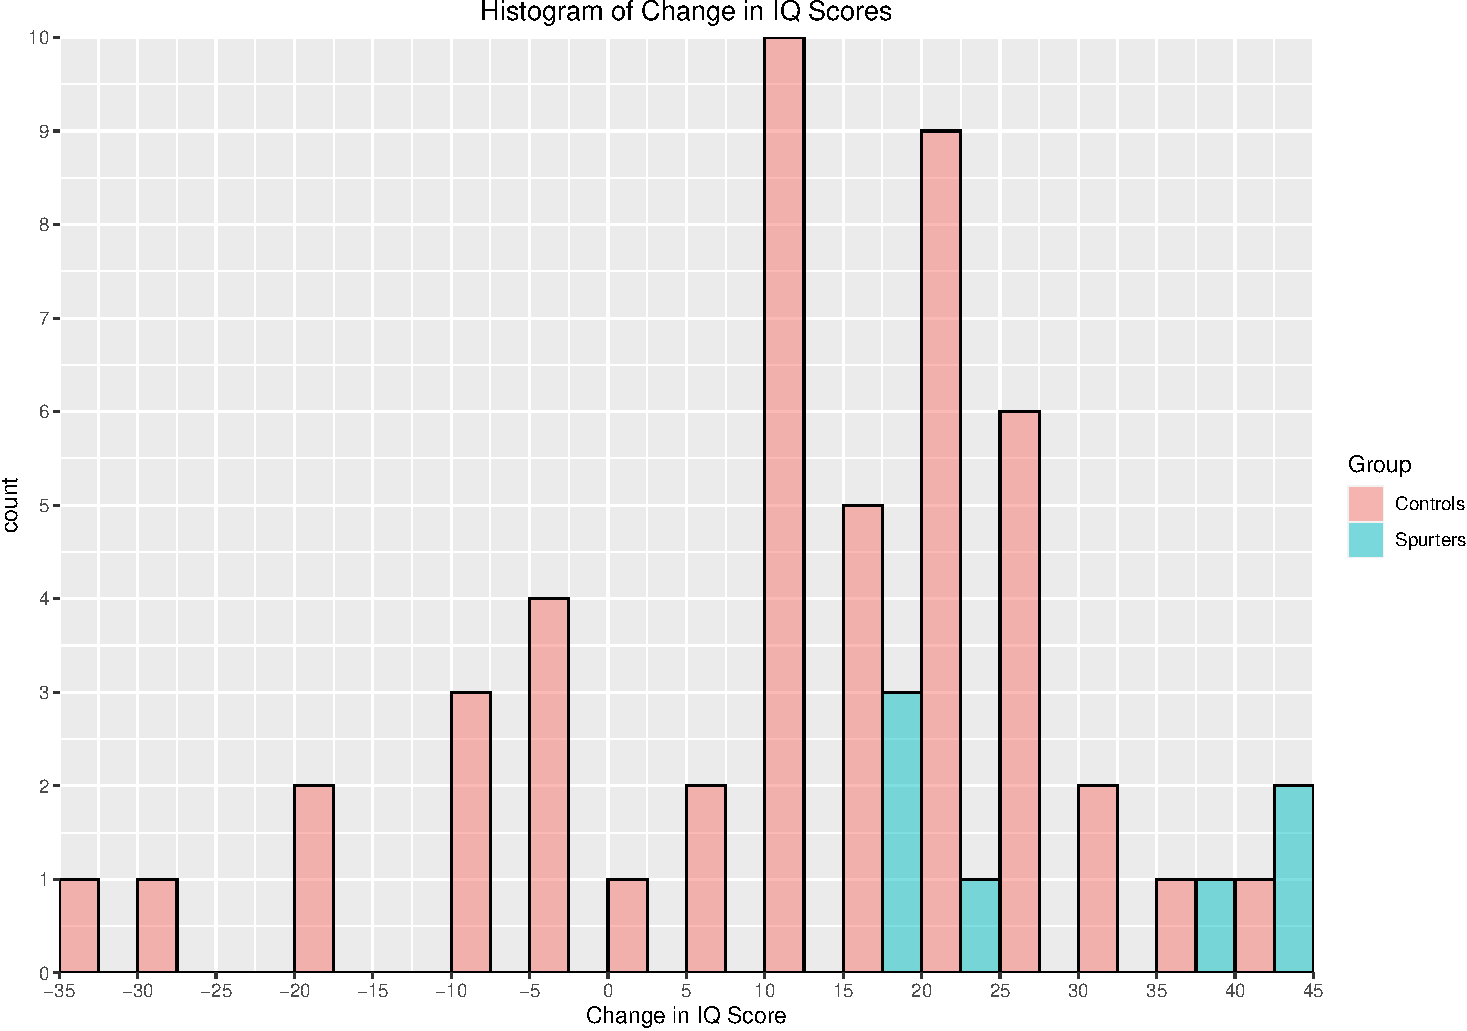
\includegraphics{04-normal-gamma_files/figure-beamer/unnamed-chunk-3-1.pdf}

\end{frame}

\begin{frame}{Histogram of Change in IQ Scores}
\protect\hypertarget{histogram-of-change-in-iq-scores-1}{}

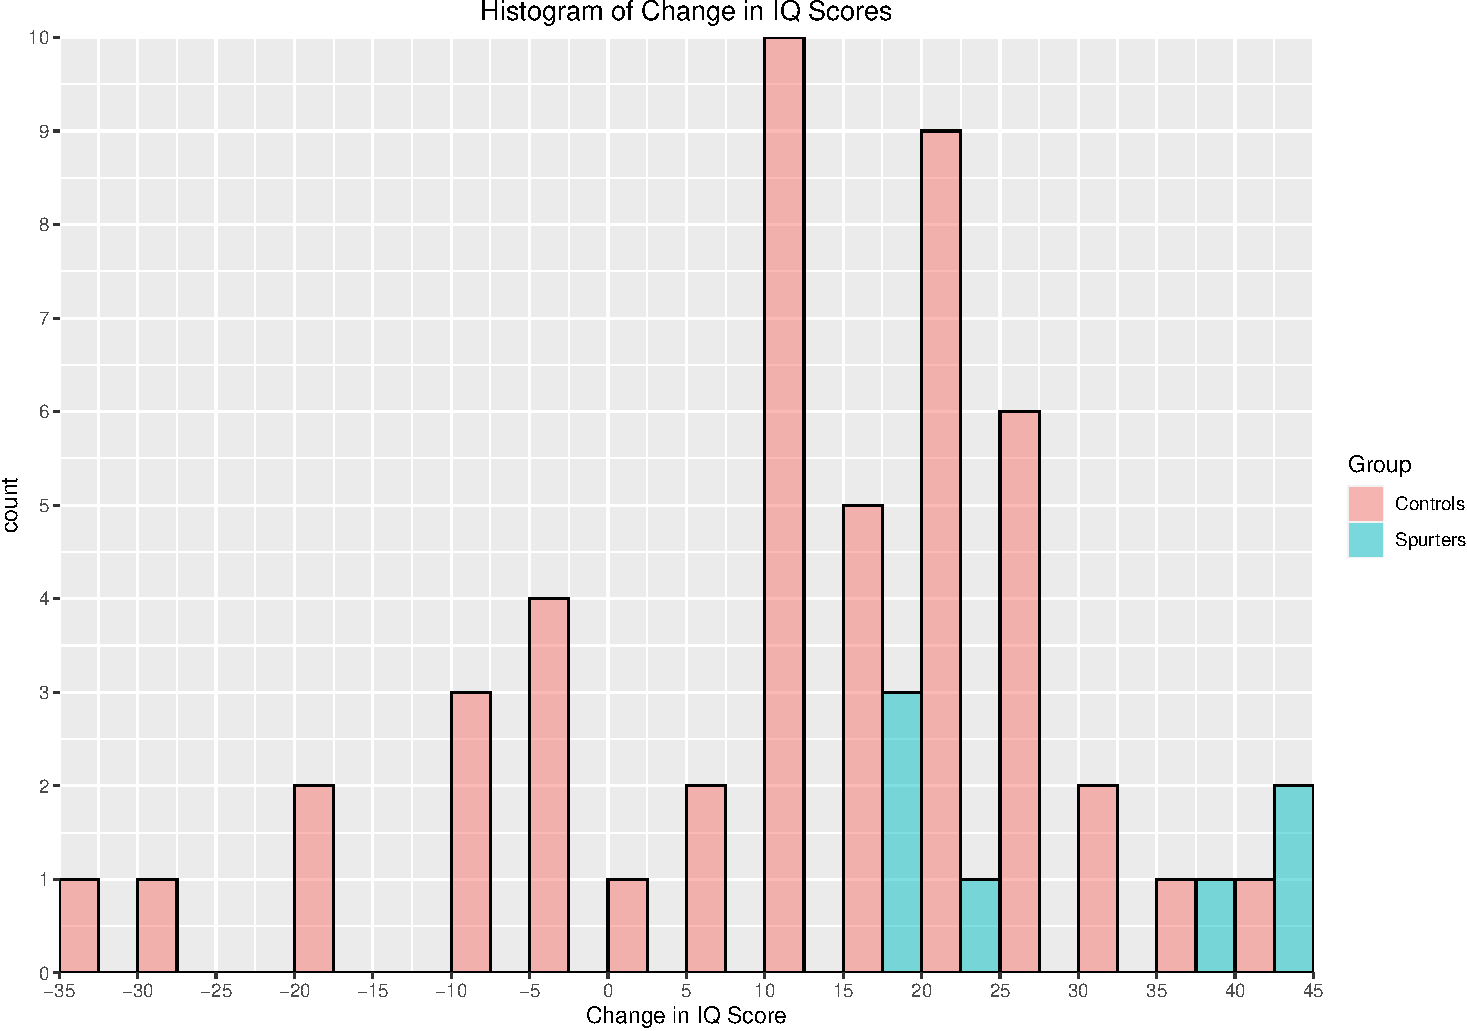
\includegraphics{04-normal-gamma_files/figure-beamer/unnamed-chunk-4-1.pdf}

\end{frame}

\begin{frame}{IQ Tests and Modeling}
\protect\hypertarget{iq-tests-and-modeling}{}

IQ tests are purposefully calibrated to make the scores normally
distributed, so it makes sense to use a normal model here:
\begin{align*}
\text{spurters: } X_1,\dotsc,X_{n_S}\iid \N(\mu_S,\lambda_S^{-1})\\
\text{controls: } Y_1,\dotsc,Y_{n_C}\iid \N(\mu_C,\lambda_C^{-1}).
\end{align*}

\begin{itemize}
\item
  We are interested in the difference between the means---in particular,
  is \(\mu_S>\mu_C\)?
\item
  We don't know the standard deviations \(\sigma_S=\lambda_S^{-1/2}\)
  and \(\sigma_C=\lambda_C^{-1/2}\), and the sample seems too small to
  estimate them very well.
\end{itemize}

\end{frame}

\begin{frame}{IQ Tests and Modeling}
\protect\hypertarget{iq-tests-and-modeling-1}{}

On the other hand, it is easy using a Bayesian approach: we just need to
compute the posterior probability that \(\mu_S>\mu_C\):
\[ \Pr(\bm\mu_S > \bm\mu_C \mid x_{1:n_S},y_{1:n_C}). \] Let's use
independent NormalGamma priors: \begin{align*}
\text{spurters: } (\bm\mu_S,\bm\lambda_S) \sim \NormalGamma(m,c,a,b)\\
\text{controls: } (\bm\mu_C,\bm\lambda_C) \sim \NormalGamma(m,c,a,b)
\end{align*}

\end{frame}

\begin{frame}{Hyperparameter settings}
\protect\hypertarget{hyperparameter-settings}{}

\begin{itemize}
\item $m = 0$ (Don't know whether students will improve or not, on average.)
\item $c = 1$ (Unsure about how big the mean change will be---prior certainty in our choice of $m$ assessed to be equivalent to one datapoint.)
\item $a = 1/2$ (Unsure about how big the standard deviation of the changes will be.)
\item $b = 10^2 a$ (Standard deviation of the changes expected to be around $10 = \sqrt{b/a} = \E(\lambda)^{-1/2}$.)
\end{itemize}

\end{frame}

\begin{frame}[fragile]{Prior Samples}
\protect\hypertarget{prior-samples}{}

\begin{verbatim}
## Warning: Removed 2139 rows containing missing values (geom_point).
\end{verbatim}

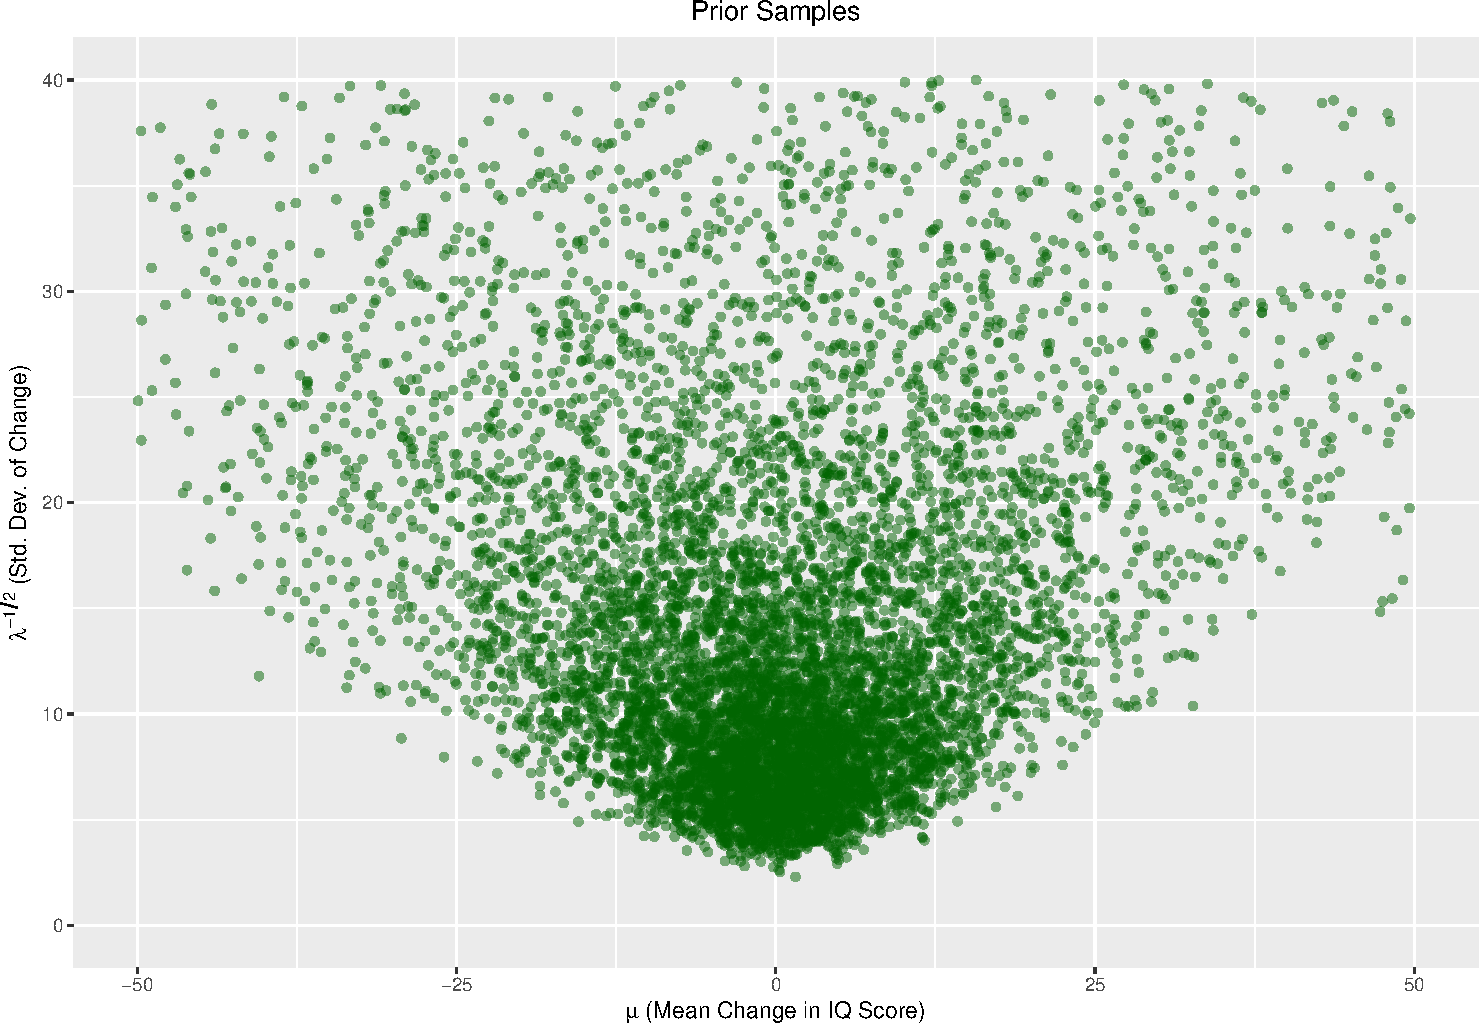
\includegraphics{04-normal-gamma_files/figure-beamer/unnamed-chunk-6-1.pdf}

\end{frame}

\begin{frame}{Original question}
\protect\hypertarget{original-question}{}

``What is the posterior probability that \(\mu_S>\mu_C\)?''

\begin{itemize}
\item
  The easiest way to do this is to take a bunch of samples from each of
  the posteriors, and see what fraction of times we have
  \(\mu_S>\mu_C\).
\item
  This is an example of a Monte Carlo approximation (much more to come
  on this in the future).
\item
  To do this, we draw \(N=10^6\) samples from each posterior:
\end{itemize}

\begin{align*}
&(\mu_S^{(1)},\lambda_S^{(1)}),\dotsc,(\mu_S^{(N)},\lambda_S^{(N)})\sim \NormalGamma(A_1,B_1,C_1,D_1)\\
&(\mu_C^{(1)},\lambda_C^{(1)}),\dotsc,(\mu_C^{(N)},\lambda_C^{(N)})\sim\NormalGamma(A_2,B_2,C_2,D_2)
\end{align*}

\end{frame}

\begin{frame}{Original question (continued)}
\protect\hypertarget{original-question-continued}{}

What are the updated posterior values?

and obtain the approximation \begin{align*}
\Pr(\bm\mu_S > \bm\mu_C \mid x_{1:n_S},y_{1:n_C}) 
\approx \frac{1}{N} \sum_{i = 1}^N I\big(\mu_S^{(i)}>\mu_C^{(i)}\big) = ??.
\end{align*}

\textbf{You will explore this more in lab 4 and homework 5.}

\end{frame}

\begin{frame}{Takeaways}
\protect\hypertarget{takeaways}{}

\begin{itemize}
\tightlist
\item
  We introduced the Normal-Gamma distribution.
\item
  We defined the precision (inverse of the variance).
\item
  We defined a hiearchical model with three levels.
\item
  We derived the posterior for the Normal likelihood and the
  Normal-Gamma prior. What did this involve?
\item
  We utilized our modeling techniques this week on an application to IQ
  scores. How realistic was this model in practice?
\item
  If you made changes to the model, what changes would you make and what
  complications might you run into?
\end{itemize}

\end{frame}

\begin{frame}{Detailed Takeaways}
\protect\hypertarget{detailed-takeaways}{}

\begin{itemize}
\tightlist
\item
  In order to understand this module, you must be able to derive the
  normal-normal model.
\item
  You must have a solid foundation regarding the normal distribution and
  its properties.
\item
  You must know the relationship between the precision and the variance.
\item
  You should be able to derive the normal-normal-gamma model.
\item
  You should conceptually understand why this model is important and
  when it's used for a case study.
\item
  You should understand conceptually what each of the four parameters of
  the normal-gamma distribution represent.
\item
  The case study for this problem (on IQ scores) is a good review
  problem regarding when you should use the normal-normal-gamma model
  over the normal-normal model. This is something that you should be
  able to conceptually walk through for this case study or a similar
  case study.
\end{itemize}

\end{frame}

\begin{frame}{Module 4 Notes}
\protect\hypertarget{module-4-notes}{}

Module 4 Class Notes can be found here:

\url{https://github.com/resteorts/modern-bayes/tree/master/lecturesModernBayes20/lecture-4/04-class-notes}

\end{frame}

\end{document}
